% JKM: adapted from Oxford Mathematical Institute
% Use one of the two documentclass lines depending on aspect ratio needed
% for 4x3 aspect ratio slides
% \documentclass{beamer}
% for 16x9 (modern wide screen) aspect ratio slides
\documentclass[aspectratio=169]{beamer}
\usetheme{uhcop}
%----------------------------------------
%          PACKAGES REQUIRED
%----------------------------------------

\usepackage{array}
\usepackage{booktabs}
\usepackage{tabularx}
\usepackage{array}
\usepackage{amsmath} 
\usepackage{xcolor}
\usepackage{ragged2e}
\usepackage{lmodern}


%----------------------------------------
%          BIBLIOGRAPHY STYLE
%----------------------------------------

%\usepackage[backend=biber,style=authoryear]{biblatex}
%\addbibresource{presentation_refs.bib} % your .bib file name here

%\RequirePackage[super,comma,numbers, sort&compress]{natbib}
\RequirePackage[authoryear,round,numbers,sort&compress]{natbib}
\bibliographystyle{unsrtnat}   % or abbrv, unsrt, alpha, unsrtnat, plainnat, etc.
\renewcommand{\bibnumfmt}[1]{[#1]}



%----------------------------------------
%          PERSONALIZE YOUR TALK 
%----------------------------------------

\title[My Talk]{\textbf{Workshop: Pharmacokinetic-Pharmacodynamics of Antimicrobials and Novel Agents}} 
\author{\href{https://www.jacobkmcpherson.com}{Jacob K. McPherson}}
\institute{
\href{https://www.uh.edu/pharmacy/about-us/academic-depts/pptr/}{Dept. of Pharmacy Practice and Translational Research} \\
\href{https://www.uh.edu/pharmacy/about-us/academic-depts/pps/}{Dept. of Pharmacological and Pharmaceutical Sciences} \\
\href{https://www.uh.edu/}{University of Houston} \href{https://www.uh.edu/pharmacy/}{College of Pharmacy}
}
\date[\today]{\today} % [short]{long for title}

%----------------------------------------
%          CONSISTENT CHAPTER TITLES
%----------------------------------------

\newcommand{\chapterone}{%
Functional and Metagenomic Evaluation of Ibezapolstat for Early Evaluation of Anti-Recurrence Effects in \textit{C. difficile} Infection
}

\newcommand{\chaptertwo}{%
Efficacy, safety, pharmacokinetics, and microbiome changes of ibezapolstat in adults with \textit{C. difficile} infection: a phase 2a multicenter clinical trial
}

\newcommand{\chapterthree}{%
The microbiome-restorative potential of ibezapolstat for the treatment of Clostridioides difficile infection...
}

\newcommand{\chapterfour}{%
Globally circulating \textit{C. difficile} are devoid of mutations associated with PolC inhibitor resistance
}

\newcommand{\chapterfive}{%

}

%----------------------------------------
%          INPUT SECTIONS OF CHAPTERS
%----------------------------------------

\begin{document}
\begin{frame}[plain]\titlepage\end{frame}
\section{Intro}
%----------------------------------------
%              INTRODUCTION
%----------------------------------------


%----------------------------------------
% Objectives Slide 
%----------------------------------------
\subsection{Objectives}
\begin{frame}[plain]{Objectives}
        \begin{enumerate} % use enumerate instead of itemize to number 
                \item
                        Describe the research into ibezapolstat-mediated microbiome restoration for the treatment of \textit{Clostridioides difficile} infection (CDI). 
                 \item
                        Posit the the non-susceptible commensal bacteria are restored via non-susceptibility to ibezapolstat. 
                 \item
                        Characterize the absence of predicted ibezapolstat resistance across globally circulating \textit{C. difficile}
        \end{enumerate}
\end{frame}

%----------------------------------------
% TERMS, ABBREVIATIONS, DEFINITIONS
%----------------------------------------
\subsection{Terminology}
% TERMS, ABBREVIATIONS -- Microbiome
\begin{frame}{Key Terms, Definitions \& Abbreviations} 
    \centering \hspace*{-1.5cm} 
    \begin{minipage}{0.95\textwidth}
        \begin{tabularx}{\textwidth}{>{\bf}l >{\footnotesize}X}
            Microbiome & The microbial biome including the ecosystem of biotic factors (e.g. bacteria, fungi), abiotic factors (e.g. viruses, metabolites), and the environment (e.g. animal intestinal tract).  \\
            Metabolome & Metabolites of the Microbiome \\
            Microbiota & Bacteria of the Microbiome \\
            CR & Colonization resistance, or the ability of commensal bacteria to prevent the colonization and overgrowth of exogenous (often pathogenic) bacteria \\
            CDI & \textit{Clostridioides difficile} infection \\
            PolC & PolC-type DNA Polymerase III alpha ($\alpha$)-subunit \\
            IBZ & Ibezapolstat, a PolC inhibitor \\
            FDX & Fidaxomicin, an RNA Polymerase inihbitor \\
            VAN & Vancomycin, a $\mathrm{D}$-\textit{Ala}--$\mathrm{D}$-\textit{Ala} bacterial cell wall biosynthesis inhibitor \\
        \end{tabularx} \tiny %text for footnote
    \end{minipage}
\end{frame}


%----------------------------------------
% BACKGROUND
%----------------------------------------
\subsection{Background}



%----------------------------------------
% COLINIZATION RESISTANCE
%----------------------------------------
%\subsection{CR}

% CONTENT SLIDE
\begin{frame}{Colonization Resistance (CR)}
    \vspace*{-10mm} % move upwards
    \begin{minipage}[t][\usableheight][t]{\usablewidth}
        \begin{columns}[T]  
            \begin{column}{0.995\usablewidth} 
                \begin{block}{\tiny\cite{van_der_waaij_colonization_1971}}
                \centering \vspace*{2mm} % move down
                    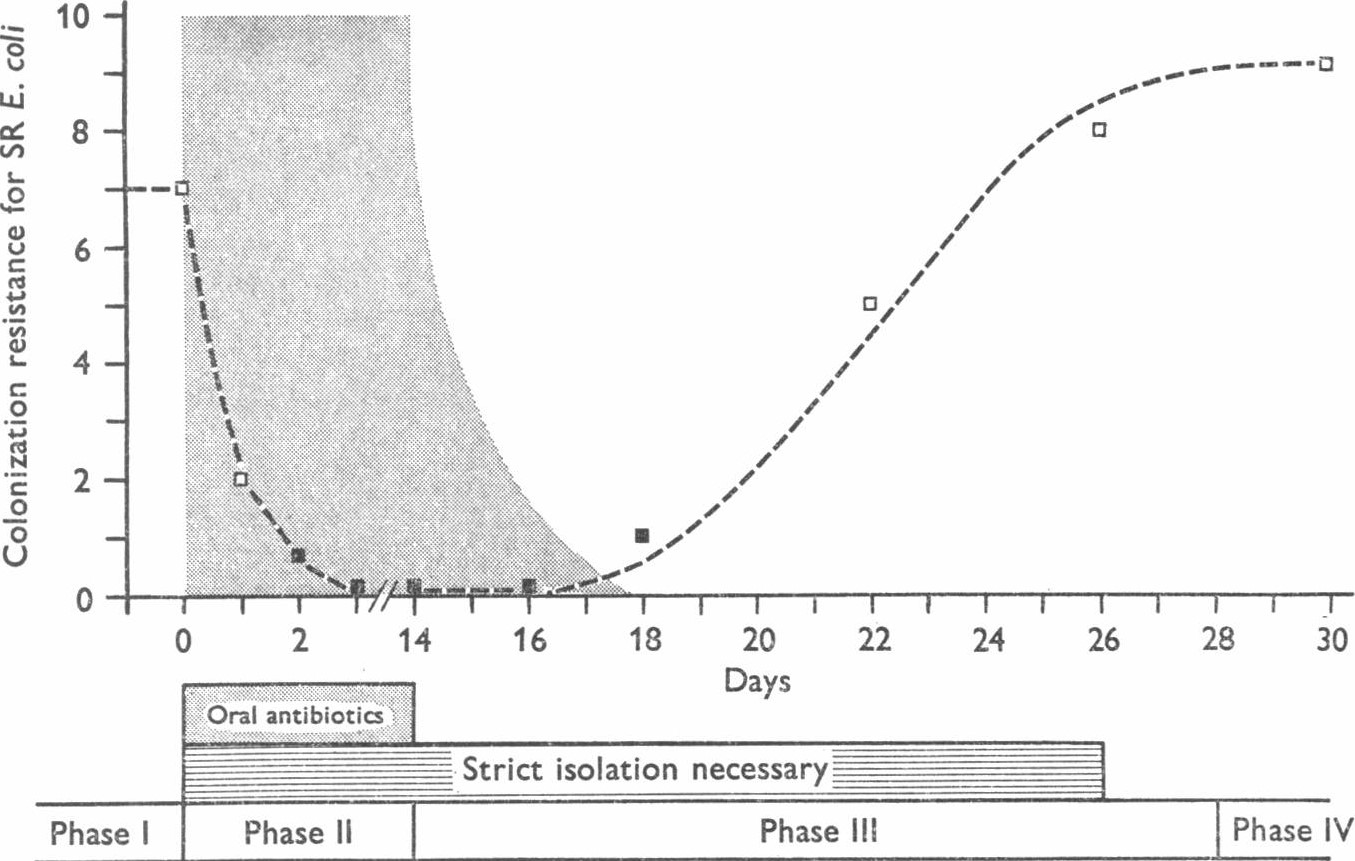
\includegraphics[
                        trim=0 0 0 0, clip,
                        width = 0.995\usablewidth, 
                        height=0.995\usableheight, % <-- Reduced to fit with block padding
                        keepaspectratio
                        ]{1971CR.jpg}
                \end{block}
            \end{column}
        \end{columns}
    \end{minipage}
\end{frame}

\ObjectivesFrameKV[ObjOne=black, ObjTwo=black, ObjThree=black]
\section{Ch.1}

% TRANSITION SLIDE
\begin{frame}[plain]
    \centering \hspace*{-1cm} \vspace*{-4cm}
        \begin{minipage}{0.8\textwidth}
            \centering
                {\usebeamerfont{section title}\usebeamercolor[fg]{section title}\LARGE
                    \textbf{Chapter 1}: \Large\textit{\chapterone}}
        \end{minipage}
        \vfill
\end{frame}



% CONTENT SLIDE
\begin{frame}{Colonization Resistance (CR)}
    \vspace*{-10mm} % move upwards
    \begin{minipage}[t][\usableheight][t]{\usablewidth}
        \begin{columns}[T]  
            \begin{column}{0.995\usablewidth} 
                \begin{block}{\tiny\cite{van_der_waaij_colonization_1971}}
                \centering \vspace*{2mm} % move down
                    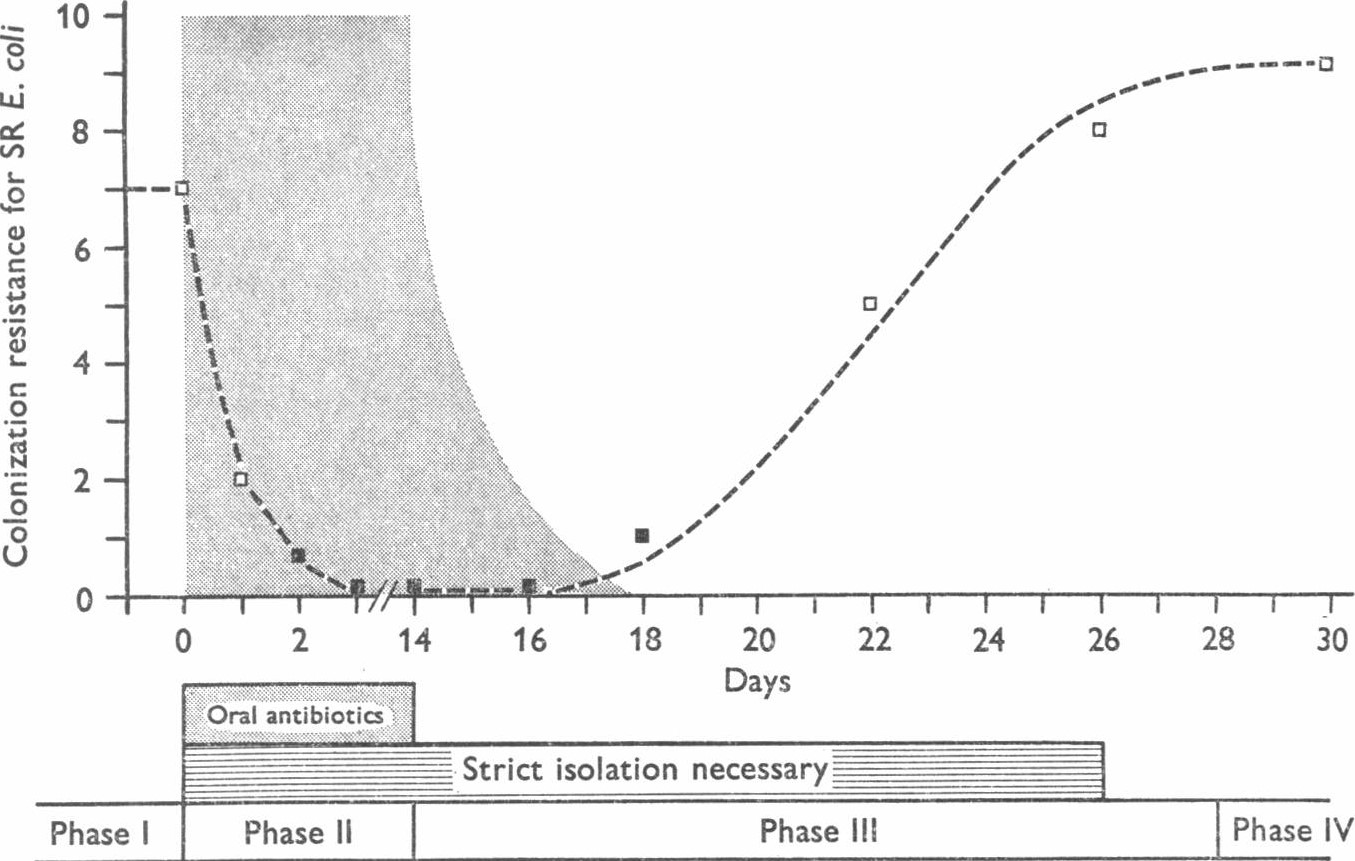
\includegraphics[
                        trim=0 0 0 0, clip,
                        width = 0.995\usablewidth, 
                        height=0.995\usableheight, % <-- Reduced to fit with block padding
                        keepaspectratio
                        ]{1971CR.jpg}
                \end{block}
            \end{column}
        \end{columns}
    \end{minipage}
\end{frame}
\ObjectivesFrameKV[ObjTwo=black, ChapTwo=black]
\section{Ch.2}% TRANSITION SLIDE
\begin{frame}[plain]
    \centering \hspace*{-1cm} \vspace*{-4cm}
        \begin{minipage}{0.8\textwidth}
            \centering
                {\usebeamerfont{section title}\usebeamercolor[fg]{section title}\LARGE
                    \textbf{Chapter 2:} \Large\textit{\chaptertwo}}
        \end{minipage}
        \vfill
\end{frame}

% CONTENT SLIDE
\begin{frame}{Colonization Resistance (CR)}
    \vspace*{-10mm} % move upwards
    \begin{minipage}[t][\usableheight][t]{\usablewidth}
        \begin{columns}[T]  
            \begin{column}{0.995\usablewidth} 
                \begin{block}{\tiny\cite{van_der_waaij_colonization_1971}}
                \centering \vspace*{2mm} % move down
                    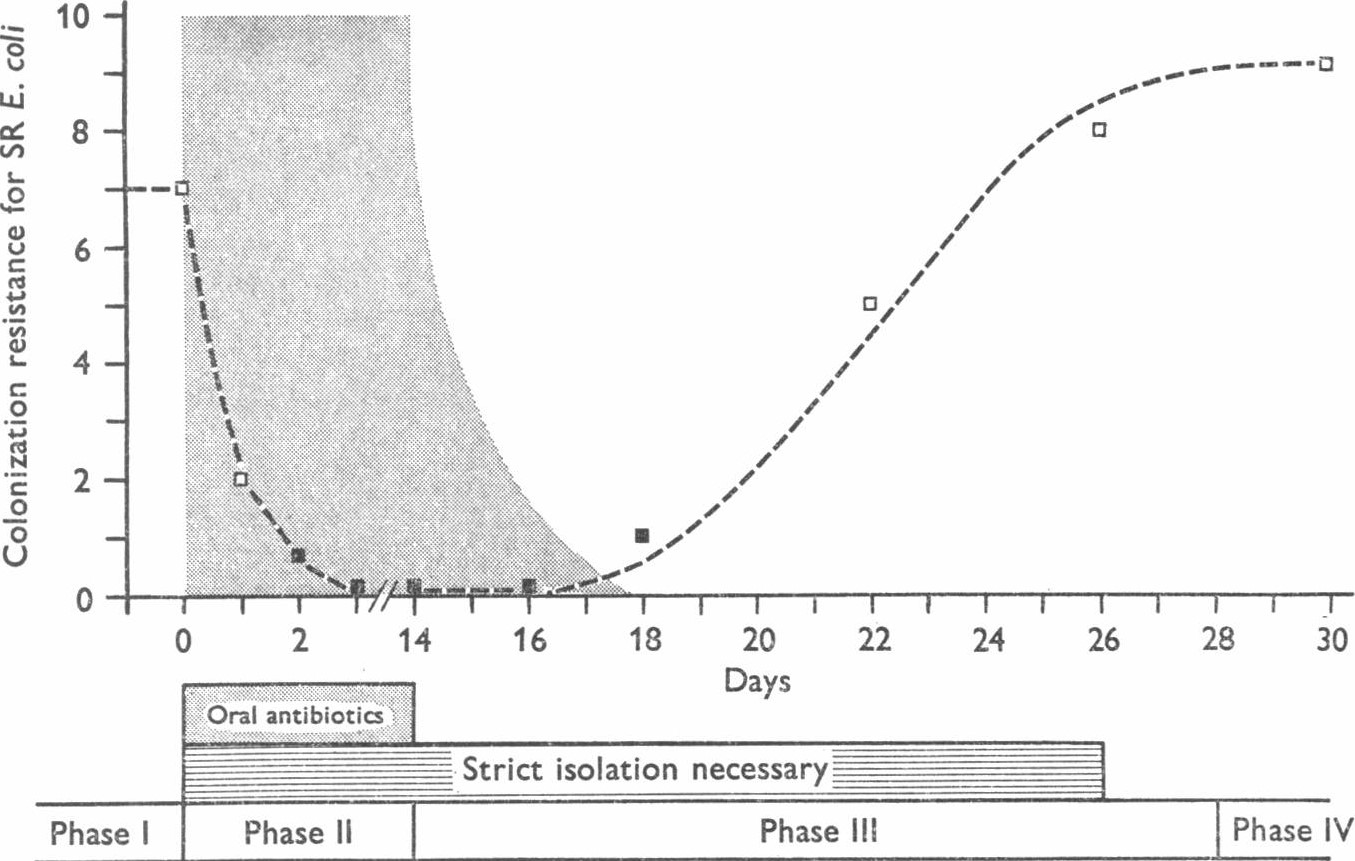
\includegraphics[
                        trim=0 0 0 0, clip,
                        width = 0.995\usablewidth, 
                        height=0.995\usableheight, % <-- Reduced to fit with block padding
                        keepaspectratio
                        ]{1971CR.jpg}
                \end{block}
            \end{column}
        \end{columns}
    \end{minipage}
\end{frame}
\ObjectivesFrameKV[ObjTwo=black, ChapThree=black]
\section{Ch.3}

% TRANSITION SLIDE
\begin{frame}[plain]
    \centering \hspace*{-1cm} \vspace*{-4cm}
        \begin{minipage}{0.8\textwidth}
            \centering
                {\usebeamerfont{section title}\usebeamercolor[fg]{section title}\LARGE
                    \textbf{Chapter 3:} \textit{\chapterthree}}
        \end{minipage}
        \vfill
\end{frame}


% CONTENT SLIDE
\begin{frame}{Colonization Resistance (CR)}
    \vspace*{-10mm} % move upwards
    \begin{minipage}[t][\usableheight][t]{\usablewidth}
        \begin{columns}[T]  
            \begin{column}{0.995\usablewidth} 
                \begin{block}{\tiny\cite{van_der_waaij_colonization_1971}}
                \centering \vspace*{2mm} % move down
                    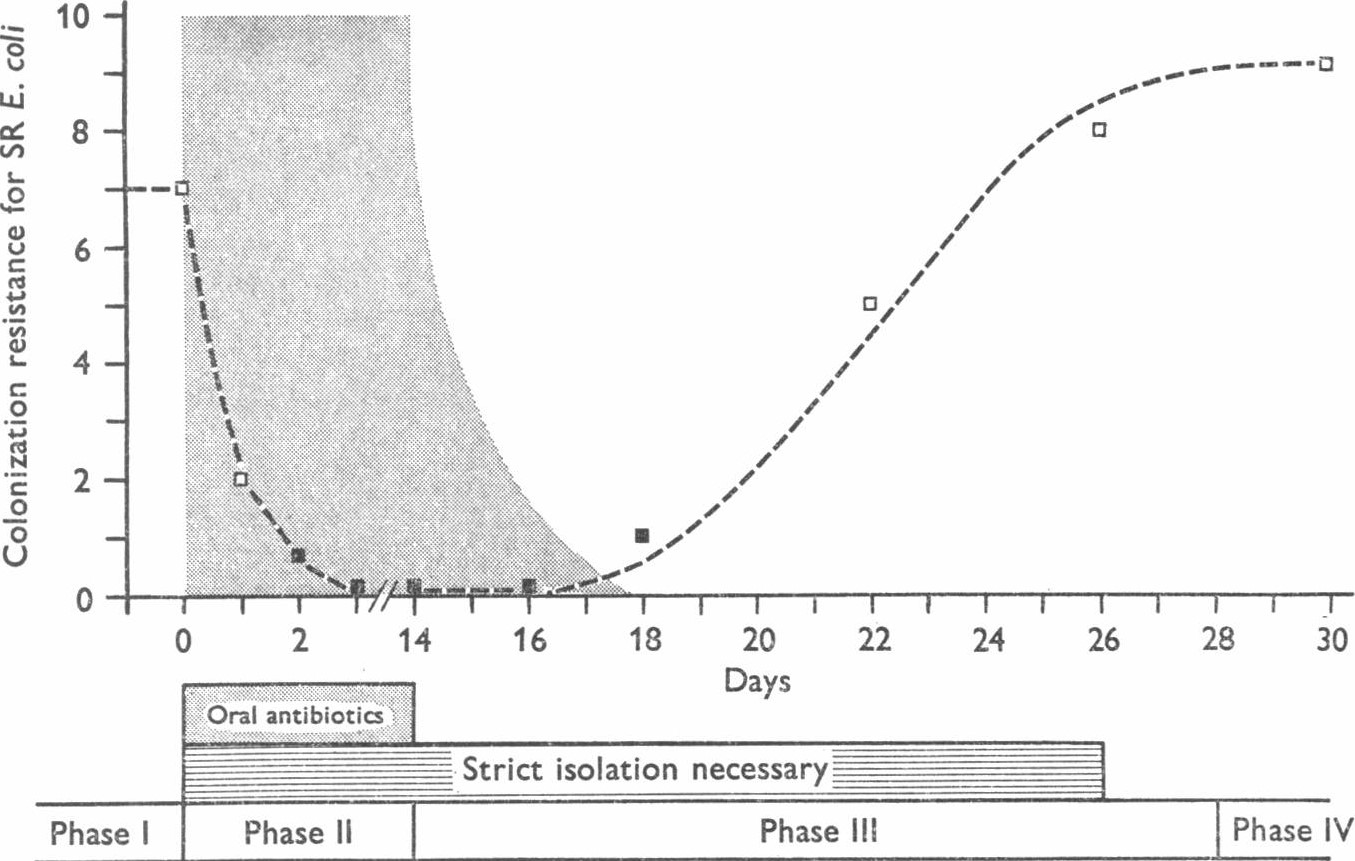
\includegraphics[
                        trim=0 0 0 0, clip,
                        width = 0.995\usablewidth, 
                        height=0.995\usableheight, % <-- Reduced to fit with block padding
                        keepaspectratio
                        ]{1971CR.jpg}
                \end{block}
            \end{column}
        \end{columns}
    \end{minipage}
\end{frame}
\ObjectivesFrameKV[ObjThree=black]
\section{Conclusion}
%--------------------------------------
%             CONCLUSION
%--------------------------------------

% TRANSITION SLIDE
\begin{frame}[plain]
  \centering
  \hspace*{-1cm}%
  \vspace*{-4cm}%
  \begin{minipage}{0.8\textwidth}
    \centering
    {\usebeamerfont{section title}\usebeamercolor[fg]{section title}\Huge What were the key takeaways?}
  \end{minipage}
  \vfill
\end{frame}

% FINAL CONCLUSION
\begin{frame}{Conclusions}

    \begin{enumerate}%[label=(\roman*)] % Roman numerals in parentheses
        \item Ibezapolstat is a PolC inhibitor with a proposed narrow-spectrum of microbiome activity in development for the treatment of \textit{C. difficile} infection, potentially restoring bacterial taxa strongly associated with colonization resistance. 
        \item Lachnospiraceae and Oscillospiraceae represent a PolC phylogenetic outgroup in the Bacillota phylum, and potentially have a variant PolC active site that renders them non-susceptible to PolC inhibitors. 
        \item Publicly available genomes of globally circulating \textit{C. difficile} are devoid of biomarkers of mutations associated with PolC inhibitor resistance. 
    \end{enumerate}
\end{frame}





% REFERENCES SLIDE

\begin{frame}{References} 
{\color{white}\cite{
% can manually insert refs not used directly in the slides, but that you want included in the bibliography
}}
\end{frame}


\begin{frame}[allowframebreaks]{References}
  %\printbibliography
  \bibliography{presentation_refs}
\end{frame}



\subsection{Acknowledgements}
% CONTENT SLIDE
\begin{frame}{Acknowledgments} \tiny
\begin{columns}[T] % Top alignment
  \begin{column}{0.3\textwidth}
    % Top-left quadrant
    \begin{block}{The Garey Lab}
      Dr. M. Jahangir Alam \\ 
      Dr. Khurshida Begum \\ 
      Dr. Chenlin Hu \\
      Dr. Eugénie Bassères \\
      Dr. Anne Gonzales-Luna \\
      Dr. Jinjee Jo \\
      Dr. Taryn Eubank \\
    \end{block}
  \end{column}
  \begin{column}{0.5\textwidth}
    % Top-right quadrant
    \begin{block}{The Committee}
      Dr. Kevin W. Garey \\
      Dr. Tahir Hussain \\ 
      Dr. Ashok Kumar \\ 
      Dr. Julian G. Hurdle \\
      Dr. Matthew L. Baker \\
    \end{block}
  \end{column}
\end{columns}
\vfill % Space between rows
\begin{columns}[T]
  \begin{column}{0.3\textwidth}
    % Bottom-left quadrant
    \begin{block}{Dept. of PPTR}
      Dr. Nicholas Beyda \\ 
      Dr. Kimberly Nguyen \\
      Dr. Nancy Ordonez \\
      Dr. Paige Pitman \\
      Dr. Dhara Surati \\
      Dr. Vincent Tam \\
      Dr. Meghna Trivedi \\
      Dr. Divya Varkey \\
      Dr. David Wallace \\
      Dr. Matthew Wanat \\
      Dr. Elisabeth Wang \\
      Dr. Austin De La Cruz \\
      Dr. Joshua Wollen \\
      Dr. Shane Tolleson \\
      Dr. Mabel Truong \\
    \end{block}
  \end{column}
  \begin{column}{0.5\textwidth}
    % Bottom-right quadrant
    \begin{block}{Dept. of PPS}
      Dr. Gregory Cuny \\
      Dr. Diana Chow \\
      Dr. Jason Eriksen \\
      Dr. Richard Bond \\
      Dr. Bradley McConnell \\
      Dr. Samina Salim \\
      Dr. MariVi Tejada-Simon \\
      Dr. Mingfu Wu \\
      Dr. Aditi Marwaha \\
      Dr. Xinli Liu \\
      Dr. Ming Hu \\
      Dr. Jiukuan Hao \\
      Dr. Krishna Boini \\
    \end{block}
  \end{column} 
\end{columns}
\end{frame}
\end{document}